\documentclass[a4paper,14pt]{extarticle}

\usepackage[utf8x]{inputenc}
\usepackage[T1,T2A]{fontenc}
\usepackage[russian]{babel}
\usepackage{hyperref}
\usepackage{indentfirst}
\usepackage{here}
\usepackage{array}
\usepackage{graphicx}
\usepackage{caption}
\usepackage{subcaption}
\usepackage{chngcntr}
\usepackage{amsmath}
\usepackage{amssymb}
\usepackage{pgfplots}
\usepackage{pgfplotstable}
\usepackage[left=2cm,right=2cm,top=2cm,bottom=2cm,bindingoffset=0cm]{geometry}
\usepackage{multicol}
\usepackage{askmaps}
\usepackage{enumitem}

\setitemize{itemsep=0em}
\setenumerate{itemsep=0em}

\renewcommand{\le}{\ensuremath{\leqslant}}
\renewcommand{\leq}{\ensuremath{\leqslant}}
\renewcommand{\ge}{\ensuremath{\geqslant}}
\renewcommand{\geq}{\ensuremath{\geqslant}}
\renewcommand{\epsilon}{\ensuremath{\varepsilon}}
\renewcommand{\phi}{\ensuremath{\varphi}}
\renewcommand{\thefigure}{\arabic{figure}} 	
\renewcommand*\not[1]{\overline{#1}}

%\titleformat*{\section}{\large\bfseries} 
%\titleformat*{\subsection}{\normalsize\bfseries} 
%\titleformat*{\subsubsection}{\normalsize\bfseries} 
%\titleformat*{\paragraph}{\normalsize\bfseries} 
%\titleformat*{\subparagraph}{\normalsize\bfseries} 

\counterwithin{figure}{section}
\counterwithin{equation}{section}
\counterwithin{table}{section}
\newcommand{\sign}[1][5cm]{\makebox[#1]{\hrulefill}}
\graphicspath{{../pics/}}
\captionsetup{justification=centering,margin=1cm}
\def\arraystretch{1.3}
\setlength\parindent{5ex}
%\titlelabel{\thetitle.\quad}

\begin{document}

\begin{titlepage}
\begin{center}
	Санкт-Петербургский Политехнический Университет Петра Великого\\[0.3cm]
	Институт компьютерных наук и технологий \\[0.3cm]
	Кафедра компьютерных систем и программных технологий\\[4cm]
	
	\textbf{ОТЧЕТ}\\ 
	\textbf{по лабораторной работе}\\[0.5cm]
	\textbf{<<Исследование персептронов>>}\\[0.1cm]
	\textbf{Нейроинформатика}\\[4.0cm]
\end{center}

\begin{flushright}
	\begin{minipage}{0.45\textwidth}
		\textbf{Работу выполнил студент}\\[3mm]
		группа 33501/4 \hspace*{10mm} Дьячков В.В.\\[5mm]
		\textbf{Преподаватель}\\[5mm]
		\sign[1.7cm] \hspace*{1mm} к.т.н., доц. Никитин К.В. \\[5mm]
	\end{minipage}
\end{flushright}

\vfill

\begin{center}
	Санкт-Петербург\\
	\the\year
\end{center}
\end{titlepage}

\addtocounter{page}{1}

\tableofcontents
\newpage
\listoftables
\listoffigures
\newpage

\section{Цели работы}

\begin{itemize}
	\item Приобретение навыков построения, инициализации и обучения НС с задержками.
	\item Исследование НС с задержками при решении задач прогнозирования зависимостей, моделируемых разностными уравнениями с конечной и бесконечной памятью.
	\item Настройка оптимальным образом количества и глубины задержек в НС.
\end{itemize}

\section{Аппроксимация линейной системы с конечной памятью}

\subsection{Формирование обучающей и тестовой выборки}

%б. Сформируйте обучающую и тестовую выборки, используя в качестве входных сигналов комбинации гармонических, случайных и ступенчато изменяющихся сигналов.
%в. Постройте графики желаемых входных и выходных сигналов для обучающей и тестовой выборок.

Сформируем обучающую и тестовую выборки на основе ранее созданных функций. На рис. \ref{fig:2_1} изображены сформированные выборки. 

\begin{figure}[H]
\begin{center}
	%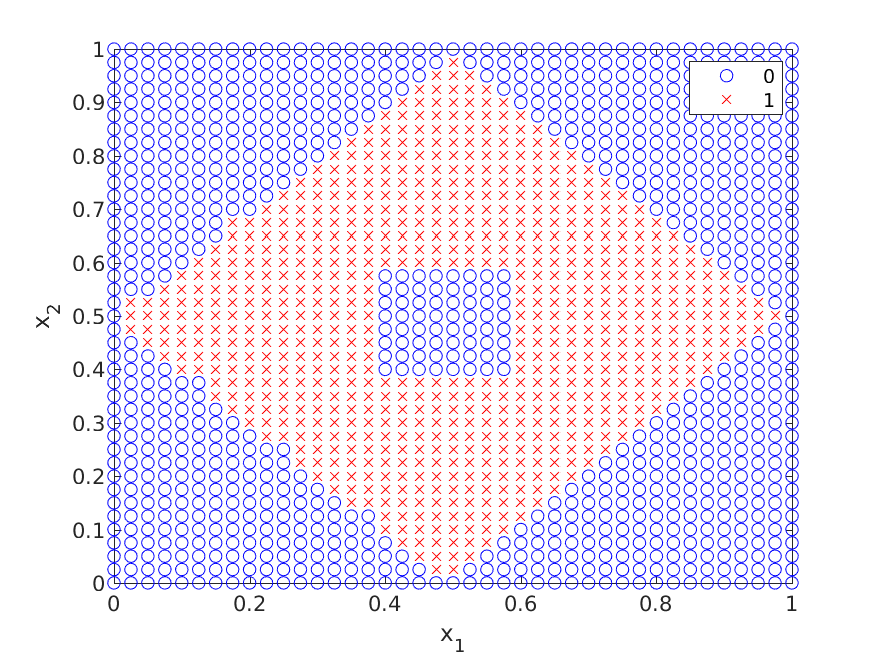
\includegraphics[scale=0.9]{2_1}
	\caption{Обучающая и тестовая выборки}
	\label{fig:2_1}
\end{center}
\end{figure}

\subsection{Обучите линейную НС}

%а. Создайте линейную НС с задержками.
%б. Задайте количество и вид задержек в соответствии с исходной линейной системой.
%в. Обучите НС на обучающей выборке.
%г. Рассчитайте ошибку на тестовой выборке и постройте графики входных и выходных (реальных и желаемых) сигналов.
%д. Приведите полученные после обучения значения весовых коэффициентов и смещений. Сравните их с коэффициентами исходной линейной зависимости.

\subsection{Изменение количества задержек}

%а. Обучите сформированные НС.
%б. Рассчитайте ошибки на тестовой выборке.
%в. Приведите полученные после обучения значения весовых коэффициентов и смещений и сравните их с коэффициентами исходной линейной зависимости.
%г. Проанализируйте полученные результаты.

\newpage

\section{Аппроксимация нелинейной системы с конечной памятью}

\subsection{Формирование обучающей и тестовой выборки}

%б. Сформируйте обучающую и тестовую выборки, используя в качестве входных сигналов комбинации гармонических, случайных и ступенчато изменяющихся сигналов.
%в. Постройте графики желаемых входных и выходных сигналов для обучающей и тестовой выборок.

Сформируем обучающую и тестовую выборки на основе ранее созданных функций. На рис. \ref{fig:3_1} изображены сформированные выборки.
\begin{figure}[H]
\begin{center}
	%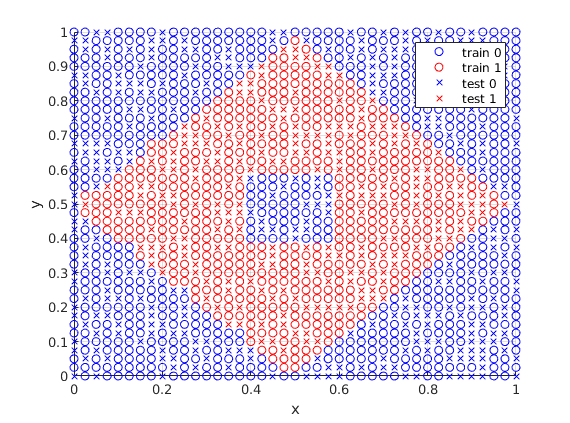
\includegraphics[scale=1]{3_1}
	\caption{Обучающая и тестовая выборки}
	\label{fig:3_1}
\end{center}
\end{figure}

\subsection{Обучение фокусированной НС с задержками}

%а. Создайте фокусированную НС с задержками, задав:
%- количество и вид задержек в соответствии с исходной нелинейной зависимостью;
%- количество скрытых нейронов, равное числу задержек.
%в. Обучите НС на обучающей выборке.
%г. Рассчитайте ошибку на тестовой выборке и постройте графики входных и выходных (реальных и желаемых) выходных сигналов.
%д. Изменяйте количество скрытых нейронов и получите усредненную зависимость ошибки на тестовой выборке от числа скрытых нейронов. Определите оптимальное количество скрытых нейронов и для него постройте графики входных и выходных (реальных и желаемых) сигналов.
%е. Попробуйте изменить количество задержек (уменьшить или увеличить), подберите оптимальные значения числа скрытых нейронов для каждого случая. Рассчитайте ошибки и проанализируйте результаты.

\subsection{Обучение распределенной НС с задержками}

%Путем подбора параметров нейронной сети:
%– числа задержек на входе;
%– количества скрытых нейронов;
%– числа задержек между скрытым и выходным слоем
%определите оптимальную конфигурацию НС, обеспечивающую минимальную ошибку на тестовой выборке и для нее постройте графики входных и выходных (реальных и желаемых) сигналов.

\subsection{Обучение линейной НС с задержками}

%В данном случае скорее всего не получится обучить НС без ошибки. Путем подбора определите оптимальное число задержек линейной НС и для него постройте графики входных и выходных (реальных и желаемых) сигналов и приведите значение ошибки.

\subsection{Сранвение результатов}

%Сравните полученные результаты для трех НС с точки зрения
%- качества аппроксимации;
%- сложности НС и времени ее обучения.

\newpage

\section{Аппроксимация системы с бесконечной памятью}

\subsection{Формирование обучающей и тестовой выборки}

%б. Сформируйте тестовые входные сигналы u[n] как комбинации ступенчатых и медленно изменяющихся гармонических сигналов с наложением случайных сигналов небольшой амплитуды.
%в. Задайте несколько комбинаций начальных условий y[0].
%г. Промоделируйте систему при сформированных значениях сигнала u[n] и начальных условиях y[0]. Постройте графики u[n],y[n].

Сформируем обучающую и тестовую выборки на основе ранее созданных функций. На рис. \ref{fig:4_1} изображены сформированные выборки: обучающая выборка обозначена ноликами, а тестовая -- крестиками.
\begin{figure}[H]
\begin{center}
	%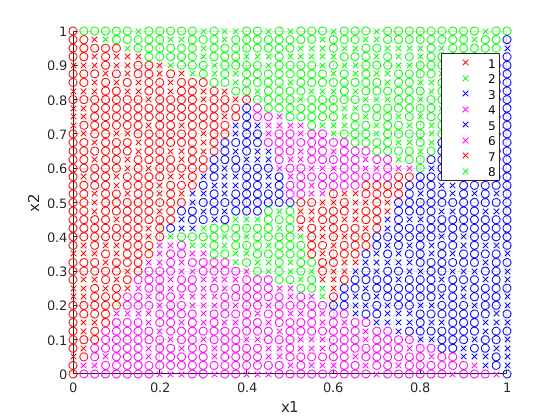
\includegraphics[scale=1]{4_1}
	\caption{Обучающая и тестовая выборки}
	\label{fig:4_1}
\end{center}
\end{figure}

\subsection{Обучение линейной НС с задержками}

%а. Изменяя количество и шаг задержек, обучайте линейную НС и определяйте ошибку на тестовой выборке. Постройте график зависимости ошибки от числа задержек.
%б. Определите оптимальное количество задержек. Для этого случая постройте графики входных и выходных (реальных и желаемых) сигналов.

\subsection{Обучение фокусированной НС с задержками}

%а. Подберите в пространстве параметров {число задержек, шаг задержек, число скрытых нейронов} их оптимальное сочетание, обеспечивающее минимальную ошибку.
%б. Для этой оптимальной комбинации постройте графики входных и выходных (реальных и желаемых) сигналов, а также значение ошибки.

\subsection{Обучение распределенной НС с задержками}

%а. Подберите в пространстве параметров {число и шаг задержек во входном слое, число и шаг задержек в скрытом слое, число скрытых нейронов} их оптимальное сочетание, обеспечивающее минимальную ошибку.
%б. Для этой оптимальной комбинации постройте графики входных и выходных (реальных и желаемых) сигналов, а также значение ошибки.

\subsection{Сравнение результатов}

%Сравните полученные результаты для трех НС с точки зрения:
%- качества аппроксимации;
%- сложности НС и времени ее обучения.

\section{Выводы}

В данной работе были приобретены навыки построения, инициализации и обучения НС с задержками для решения задач прогнозирования зависимостей, моделируемых разностными уравнениями с конечной и бесконечной памятью. Была проведена настройка оптимальным образом количества и глубины задержек в НС.

\end{document}